% Working introduction (will probably replace all of it)
% \section{Introduction}

\noindent
There's a question on my mind, that is perhaps best represented in the manner of a dialogue. It's a question on the nature of consciousness, where we ask not only: \emph{What is consciousness?}, and \emph{where is consciousness located?}. But in order to do so, we must first explore adjacent questions in ontology, like \emph{what is being?} or \emph{what is meaning?} I will develop these questions in the course of this dialogue, which I present as follows.

% \begin{table}[H]
%   \centering
%   \begin{tabular}{@{}ll@{}}
%     \toprule
%     \multicolumn{2}{l}{Dramatis personae}  \\ \midrule
%     \textsc{You}     & \textit{the Reader} \\
%     \textsc{Visitor} & \textit{the Other}  \\
%     \textsc{I}       & \textit{the Author} \\ \bottomrule
%   \end{tabular}
%   \label{tab:characters}
% \end{table}

Imagine one day, a \textsc{Visitor} arrives to your office. You offer them tea, and after all the introductions and customary salutations, they inquire of you the following question: "What is chess?", they ask.

Of course, you would be astonished -- for how could they not know of such a common game? But your \textsc{Visitor} hails from a faraway land, with no knowledge of your customs. So despite your bemusement, you proceed with an impromptu demonstration. You find a dusty chess-board beneath some papers, and a box of chess-pieces behind a shelf. Presenting these materials to your \textsc{Visitor}, you arrange the pieces in their starting order, and explain the movements of the chess-pieces. You showcase the forward marching of the Pawns, and the odd, L-shaped pounces of the Knight. Thus you demonstrate the pieces one-by-one, as well as other nuances of the rules, such as checkmate and \emph{en passant}.

After you conclude your explanation, you look expectantly at your visitor. They seem surprised. "What a marvellous invention of yours, this `chess'!", they exclaim. "And surely, you have a prized possession indeed, for many strangers to speak of its renown. But should anyone else wishes to see this game, must they also come visit you at your office, just as I have done?"

You laugh, bemused by your \textsc{Visitor}'s peculiar misunderstanding. You quickly explain. No, you were not the inventor of chess (if only!). Nor is your worn-out chess board \emph{the} `Chess' of the world. In fact, you clarify -- your visitor has confused the \emph{singular} with the \emph{general}. There are such things which are singular, such as You and I (or the Eiffel Tower). And in English, we often denote their singularity with the definite article -- "\emph{the} Eiffel tower, not \emph{an} Eiffel tower". But in any case, chess is a game that is enjoyed by millions, of which you only possess a particular instance -- namely that battered chess-board which is now in front of you both.

% A Materialist Foundation for Being
% \section{A Material Foundation for Being}


Your \textsc{Visitor} looks thoughtful, and glances at the chess-board, with an odd intensity. After they moment, state pensively: "So chess is not this \emph{particular} board and these \emph{particular} pieces which you have in front of you." You nod, encouragingly. They pick up a Rook, and examine it -- before proceeding: "But rather, chess is a game of black and white pieces, made from ebony and boxwood. It is played on a varnished, mahogany board, with black and white squares made from oak and birch."

"And hence, anyone may possess a particular instance of chess, should they own a board and a piece-set constructed by these materials and dimensions," they conclude.

You object, stating that they have misunderstood once again. No, chess is not defined by these material characteristics. A game of chess is not defined by ebony and boxwood pieces, nor must a chessboard be made from mahogany, oak, and birch. Rather, there can be chessboards made from plastic or canvas, chess-pieces from metal or glass. Indeed, there is no necessity for the pieces to be black and white either -- all of these are merely material characteristics which are \emph{accidental} to the essence of chess altogether. To define the \emph{being} of chess as a set of material properties would miss what is essential about chess. To drive forth the point, you make sure to recount a rather charming miniature chess-set you saw, made from frosted and transparent crystal -- at a colleague's office down the hall.

The \textsc{Visitor} remains silent for a few moments, taking this all in. "Chess is not defined by its material characteristics, but rather it's material characteristics are accidents from any particular embodiment of it's being." You nod along, reasonably. They look up at you, with a look of increasing bafflement. "But then, what \emph{is} chess?!"

% \section{A Logical Foundation for Being}

You lean back in your armchair, taking a moment this time to ponder. You arrive at an answer, presenting it this time with more care. Chess is not defined by any material characteristics of its components, you admit. But rather, a board game is chess, when its pieces follows certain definite rules. A chess-game is a game where there is a board composed of 64 alternating squares, arranged in an eight-by-eight grid. Where each player controls sixteen pieces, eight of which are Pawns. You generalise even further, making sure to point out that it is not necessary for the pieces and squares to be black and white -- nor any colours at all, provided that they are differentiated from each other. And likewise, it is not necessary for the pieces to be `Pawns,' `Bishops,' `Knights,' and `Kings' -- the customary names that we give them are also accidental. Instead, their true natures are defined by their movements.

A contemplative silence settles over the both of you. Your \textsc{Visitor} considers your explanation with an unusual attentiveness. After a while, they speak.

"You state that chess a general being, which manifests in particular instances. It is not defined by the material characteristic of these instances, but rather by a set of underlying rules which define certain behaviours."

The \textsc{Visitor} looks puzzled, and pauses for a moment before they exclaim: "But now that you divorce the definition of chess from the material basis of its embodiment, you risk a progression into absurdity!"

Astonished, you interject -- and ask what them what they mean.

"If chess were to be defined as a set of logical rules, these rules may be present under any representation. You would not need a chess board, or chess pieces at all, in order to have chess!"

You laugh, surprised by the \textsc{Visitor}'s particular objection. Why, you say-- that is not a problem at all. Indeed, chess is represented -- and played -- often without chess boards nor chess pieces. You mention the existence of correspondence chess -- matches played via post or internet forums, where nary a chess-board is in sight. You present the concept of Descriptive Chess Notation, a terse, succinct language that's often used to represent chess matches in print. To better illustrate this, you even print off an example, of the opening moves from a match between two Grandmasters in Berlin\footnote{The \href{https://en.wikipedia.org/wiki/Evergreen_Game}{\emph{Evergreen Game}}, a famous chess match between Adolf Anderssen and Jean Dufresne in 1852.}:

\begin{figure}[H]
  \begin{center}
    \fbox{
    \begin{minipage}{0.5\textwidth}
      \NumTabs{8}
      \vspace{5mm}
      \begin{enumerate}
        \item \texttt{P-K4\tab P-K4}
        \item \texttt{N-KB3\tab N-QB3}
        \item \texttt{B-B4\tab  B-B4}
        \item \texttt{P-QN4\tab BxNP}
        \item \texttt{P-B3\tab  B-R4}

        \ldots
      \end{enumerate}
    \end{minipage}
  }
  \end{center}
  \caption{Descriptive Chess Notation}
  \label{fig:DCN}
\end{figure}

\noindent
Your \textsc{Visitor} studies the printout closely. "I do not see the chess-pieces," they state. "Nor how there is any movement in space."

Ah, but you are simply unaccustomed to reading Descriptive Chess Notation, you reassure. For you see, each numbered line in the printout represents a pair of moves, the first belonging to white, the second to black. Each move contains a letter and a destination square, where P represents `Pawn', N represents `Knight', and so on. Given the expression "\texttt{P-K4}", it would mean "move the (white) Pawn to the fourth square in front of the (white) King". It's all a little obscure, but to an experienced chess player reading such notation is as clear as seeing a movie play out in their mind.

"I see," nods the \textsc{Visitor}. They revisit the printout, which now appears with a newfound significance.

"From what I understand so far, the essence of chess is not in its material embodiment. But rather, it is a set of rules, and relations, which may manifest within an arbitrary set of \emph{symbols} which represent them. These symbols may be totems of carved ebony and boxwood, or simply letters upon a page."

"But in both cases, the simple symbols by themselves are not enough to be chess. To a person that does not know about Descriptive Chess Notation, your printout will have the appearance of random, meaningless characters. Likewise, boxwood chess-pieces would look like simple wood-turnings to a person ignorant of their use."

% \section{A Symbol-Interpretation Foundation for Being}

You agree to your \textsc{Visitor}'s elaboration. Perhaps, you muse provisionally -- there are two components to the being of chess. There is, by necessity -- a set of symbols which represent the state of the game. But there must also be a corresponding \emph{interpretation}, which inscribes \emph{meaning} to the symbols. In fact, you hypothesise, there is probably a formal method to define the being of chess, as a set of symbols and a suitable interpretation.

"Like a formal language. Where the alphabet is a set composed of the chess pieces, and a grammar which defines valid combinations of moves."

Or a geometrical system, you reply. One which contains definitions of the chess-pieces, and postulates which allow their moves.

(Or even a Turing-machine, I add, narrating from the margins. But that is neither here nor there. The dialogue continues on.)

You feel there's a certain oddity with this definition of chess, and your \textsc{Visitor} notices it too, who takes it upon themselves to elaborate:

"We've arrived at a puzzling stopping-point, in this progression of abstraction", they state. "We began with wooden chess-pieces, physical and embodied -- as real objects with extension in space and time. We than divorce chess from it's material representation, and ultimately conclude that it's essence lays in a set of symbols and a suitable interpretation."

\textsc{The Visitor} picks up a pen and makes a few notes on the printout. "For the sake of convenience, let us denote the set of symbols as $\{\text{Symbols}\}$, and their interpretation as a function $I(x)$. The process of interpreting symbols to yield meaning can be written as:"

\begin{equation*}
  \{\text{Symbols}\} \Rightarrow I(x) \Rightarrow \{\text{Meaning}\}
\end{equation*}

So given a collection of symbols like the printout from above (\autoref{fig:DCN}), there exists a suitable interpretation that yields meaning from otherwise obscure lines. You grant this step of reasoning.

"But these symbols and their interpretation may be of arbitrary complexity," they frown. "By going further in abstraction, we encounter the same absurdity that I feared earlier."

What sort of absurdity? You ask the \textsc{Visitor} to clarify, and they provide an example:

% \section{Extending the Symbol-Intepretation Hypothesis}

"Let me take your earlier representation of a chess match, in Descriptive Chess Notation (\autoref{fig:DCN}). I will make some minor changes to the representation, for the sake of demonstration." They pick up your printout and a proffered pen, and begin to write. "I will replace the arabic numbers with their numerals, and remove any dashes and space. With these minor, purely notational substitutions, the match takes on the following form."

You glance at their amendations:

% Plaintext, Encryption Key, Ciphertext for example
% PKFOURPKFOURNKBTHREENQBTHREEBBFOURBBFOURPQNFOURBXNPPBTHREEBRFOUR
% DTUMRBIMJVAPEIXYMJUOWYLSMGKLTWGYJXQWGTBKMBQUGTPXVJGJVKTODURMBCQX
% SDZALSXWOJUGRSYRTAYSJOMLTXOPUXLMDORXLHVBBRDZUNGYSWVYWDAFHYSDGQKO

% Plaintext, Encryption Key, Ciphertext for full game
% PKFOURPKFOURNKBTHREENQBTHREEBBFOURBBFOURPQNFOURBXNPPBTHREEBRFOURPQFOURPXPOOPQSIXQNTHREEQBTHREEPKFIVEQNTHREERKONEKNKTWOBRTHREEPNFOURQXPRQNONEQRFOURBNTHREEQNQTWOBNTWONKFOURQBFOURBXQPQRFOURNBSIXchPXNPXPRNONEQRQONEQXNRXNchNXRQXPchKXQBBFIVEdblchKKONEBQSEVENchKBONEBXNMATE
% DTUMRBIMJVAPEIXYMJUOWYLSMGKLTWGYJXQWGTBKMBQUGTPXVJGJVKTODURMBCQXOFCCRPILTLDVZNUSGUIXBQQXQTSPEKIGJZZDEQPXWTVHSFZTVJJLVNBSIZDZYASDWROOZHCCHXDBCXPCQMHSBHTIQCMDSUSYETSGWREPUPHHDBLEEXCTDNEQMVQSRNNXXOUVXZUORDUREZTCOQCSORKWFSXEOBUJEEJIQDVFYHHXMOIUPSPRSJFFXMMQFEONUYPRXRSJPZ
% SDZALSXWOJUGRSYRTAYSJOMLTXOPUXLMDORXLHVBBRDZUNGYSWVYWDAFHYSDGQKODVHQLGXIIZRKPFCPWHBESUUNRMZGIOXQOHUHUDIENXZYCTMXFWTERBCJBGUDCPFIKLFEWWTSULQFSOUQKDIFUOKMUSZTLQGZRMOUJBJDOGXIIPFVFUSITEJEGMDTJVKZEDRIMWJFERHVUQJQBUSPBIHJHZKBFRRYGLTFGEWKGCLANZKBZCDEWKVXBHQDHLYOILTSUEEJID

\begin{figure}[H]
  \begin{center}
    \fbox{
    \begin{minipage}{0.5\textwidth}
      \begin{center}
        \vspace{5mm}

        \texttt{PKFOURPKFOURNKBT}

        \texttt{HREENQBTHREEBBFO}

        \texttt{URBBFOURPQNFOURB}

        \texttt{XNPPBTHREEBRFOUR}

        \ldots
      \end{center}
    \end{minipage}
    }
  \end{center}
  \caption{Modified Descriptive Chess Notation}
  \label{fig:DCN-mod}
\end{figure}

"With this string of characters (i.e. symbols), there exists an interpretation such that they yield a chess game. This is not difficult to grant, for the string is a simple, idiosyncratic variation on Descriptive Chess Notation," the \textsc{Visitor} explains.

What an ungainly representation. But it can be done, you allow.

"But now I will do the following. I will take the above string and encrypt them with a password according to a cypher, yielding an encrypted output."

You raise a puzzled eyebrow.

"A cypher can be understood as a simple, reversible function, which takes a key and an input." The \textsc{Visitor} clarifies. "If you input plaintext and the key, it's output will be ciphertext. If you input ciphertext and the (correct) key, it will output the original plaintext." They helpfully scribble down some notation.

\begin{align*}
  C(k, i) &= O \\
  C(k, \text{plaintext}) &= \text{ciphertext} \\
  C(k, \text{ciphertext}) &= \text{plaintext}
\end{align*}

What does this have to do with symbols and interpretation, you ask.

"The philosophical import of this example comes from the following cryptographic principle. Any good cypher is capable of producing seemingly random ciphertext, given an input and an appropriate key. Given the modified notation as input, and a well-chosen cipher and key\footnote{The specific cipher used in this example is a one-time-pad.}, I can produce the following ciphertext as output:"

\begin{figure}[H]
  \begin{center}
    \fbox{
    \begin{minipage}{0.5\textwidth}
      \begin{center}
        \vspace{5mm}

        \texttt{SDZALSXWOJUGRSYR}

        \texttt{TAYSJOMLTXOPUXLM}

        \texttt{DORXLHVBBRDZUNGY}

        \texttt{SWVYWDAFHYSDGQKO}

        \ldots
      \end{center}
    \end{minipage}
    }
  \end{center}
  \caption{Encrypted Descriptive Chess Notation}
  \label{fig:DCN-crypt}
\end{figure}

You examine the result, comparing to the earlier plaintext string (\autoref{fig:DCN-mod}). It does look pretty random, you admit. Any appearance of structure and meaning seems to be obliterated.

"But here's the thing. This string does not only have the mere \emph{appearance} of randomness. But it \emph{is} truly random, by all mathematical measures. You can give it to a Mathematician, who could subject it to exacting statistical analysis. They will find that the frequency distribution (i.e. occurances) of letters will be uniform and evenly distributed. The encrypted string will be mathematically indistinguishable from random noise."

You let the \textsc{Visitor}'s words sink in for a moment.

But this is such a pedestrian objection! You protest.

You still have a set of symbols, and a corresponding interpretation. The only difference is that the symbols are obfuscated, by adding a cryptographic key and decryption step to the interpretation. Sure, one may add any number of steps and contrivances in the interpretation, but it doesn't change the essential nature of chess as symbols and a means to interpret them.

% \section{The \emph{Reductio ad Absurdum}}

"I apologise, but you misunderstood my point", replies the \textsc{Visitor} good-naturedly.

"For the essential structure of my syllogism is thus. Given a set of symbols and an interpretation, I can yield meaning, as agreed upon before."

\begin{equation*}
  \{\text{Symbols}\} \Rightarrow I(x) \Rightarrow \{\text{Meaning}\}
\end{equation*}

"With the deciphering process, I essentially add an additional step in the process. First, the cipher-function $C(x)$ takes a meaningless input, which yields the symbols that are then interpreted by $I(x)$."

\begin{equation*}
  \{\text{No Meaning}\} \Rightarrow C(x) \Rightarrow \{\text{Symbols}\} \Rightarrow I(x) \Rightarrow \{\text{Meaning}\}
\end{equation*}

"You are right to admit, however -- that the additional deciphering process is not essentially different from interpretation. It is merely a continuation (or rather, an extension) of the interpretive act. Indeed, it can be simplified into it, where $I'(x) = I(C(x))$, just like functions can be composed (i.e. nested)"

\begin{equation*}
  \{\text{No Meaning}\} \Rightarrow \underbrace{ \big[ C(x) \Rightarrow \{\text{Symbols}\} \Rightarrow I(x) \big] }_{I'(x)} \Rightarrow \{\text{Meaning}\}
\end{equation*}

\noindent
"And thus, we yield the conclusion of our \emph{reductio ad absurdum}. Given something that is meaningless, there exists a suitable interpretation $I'(x)$ which yields a meaning."

\begin{equation*}
  \therefore \{\text{No Meaning}\} \Rightarrow I'(x) \Rightarrow \{\text{Meaning}\}
\end{equation*}

"Not only that, but given something which has no meaning, there will always exist a suitable interpretation of it which can yield an arbitrary meaning of one's choice. For any string of random characters, there can be an interpretation that yields a riveting novella. Within any noise of radio static, there is a suitable interpretation that yields a lost concerto of Bach."

But this is an absurdity! You protest. By stretching the nature of symbols and their interpretation to such an extreme, we risk losing meaning entirely. There has to be some paralogism in this chain of reasoning, or some illusion at hold. Otherwise, it seems that the very structure of being loses its shape. How can we affect an explanation?

"We can try. For one, the absurdity of this conclusion comes an imbalance between the symbols and interpretation." The \textsc{Visitor sighs}. "We hollow out the symbols until there is nothing left within them, just as we simultaneously over-stuff the interpretation so that it does all the work. But yet, somehow meaning is conserved in the two parts as a whole -- it is merely distributed unevenly."

\begin{figure}[H]
  \centering
  \begin{tikzpicture}
    % Complete Rectangle #1
    \tkzDefPoint(0,0){A}
    \tkzDefPoint(3,0){B}
    \tkzDefPoint(0,3){C}
    \tkzDefPoint(3,3){D}
    \tkzDrawPolygon(A,B,D,C)
    % Larger slice
    \tkzDefPoint(0,2){E}
    \tkzDefPoint(3,2){F}
    % \tkzLabelPoints(E,F)
    \tkzDrawPolygon(A,E,F,B)
    % Midpoints
    \tkzDefMidPoint(A,B) \tkzGetPoint{AB}
    \tkzDefMidPoint(E,F) \tkzGetPoint{EF}
    \tkzDefMidPoint(C,D) \tkzGetPoint{CD}
    % Centers
    \tkzDefMidPoint(AB,EF) \tkzGetPoint{BigCenter}
    \tkzDefMidPoint(EF,CD) \tkzGetPoint{SmallCenter}
    \tkzLabelPoint[align=center,anchor=center](BigCenter){Complex \\ Intepretation}
    \tkzLabelPoint[align=center,anchor=center](SmallCenter){Simple \\ Symbols}
    % \tkzDrawPoints(A,B,C,D)
    \tkzDrawPolygon(A,B,D,C)
    % \tkzLabelPoints(A,B,C,D)

    % Complete Rectangle #2
    \tkzDefPoint(4,0){A'}
    \tkzDefPoint(7,0){B'}
    \tkzDefPoint(4,3){C'}
    \tkzDefPoint(7,3){D'}
    \tkzDrawPolygon(A',B',D',C')
    % Smaller slice
    \tkzDefPoint(4,1){E'}
    \tkzDefPoint(7,1){F'}
    % \tkzLabelPoints(E',F')
    \tkzDrawPolygon(A',E',F',B')
    % Midpoints
    \tkzDefMidPoint(A',B') \tkzGetPoint{AB'}
    \tkzDefMidPoint(E',F') \tkzGetPoint{EF'}
    \tkzDefMidPoint(C',D') \tkzGetPoint{CD'}
    % Centers
    \tkzDefMidPoint(AB',EF') \tkzGetPoint{BigCenter'}
    \tkzDefMidPoint(EF',CD') \tkzGetPoint{SmallCenter'}
    \tkzLabelPoint[align=center,anchor=center](BigCenter'){Simple \\ Intepretation}
    \tkzLabelPoint[align=center,anchor=center](SmallCenter'){Complex \\ Symbols}
    % \tkzDrawPoints(A,B,C,D)
    \tkzDrawPolygon(A',B',D',C')
    % \tkzLabelPoints(A',B',C',D')

    % Equal Sign
    \tkzDefMidPoint(B,A') \tkzGetPoint{Mid1}
    \tkzDefMidPoint(D,C') \tkzGetPoint{Mid2}
    \tkzDefMidPoint(Mid1,Mid2) \tkzGetPoint{Mid3}
    \tkzLabelPoint[align=center,anchor=center](Mid3){$=$}
  \end{tikzpicture}
  \caption{Illustration of Meaning, as Symbols and Interpretation}
  \label{fig:meaning}
\end{figure}


You nod. There's a similar meta-theorem in the study of Hilbert-style logic systems, you recall. Given a logical system with axioms, and rules of inference -- there is always some tenuous balance in play. You can either have a system that has few axioms, but many rules of inference. Or a system that has many axioms, but few rules of inference. It seems like a similar dynamic is at play here.

But still, there is no reconciliation yet. If anything, all this goes to illustrate is that the conception of chess (or anything) as a set of symbols and an interpretation is an illusion. After all, meaning is still conserved -- no matter how you distribute the share of work between symbols and the interpretative function (\autoref{fig:meaning}).

You both ponder now, in silence. All of a sudden, the office feels chilly and strange. There is such a thing as chess, that is certain. Chess is a well-defined being which exists. It's trivial to dismiss the \emph{material cause} as a definition, but now it seems that the \emph{formal cause} is just as useless in explaining what being (or chess, for that matter) is. You feel a sense of \emph{aporia} set in, as your \textsc{Visitor} politely shifts in the armchair.

"If I may," the \textsc{Visitor} offers gently. "I think there's something hidden here. Not in the interpretative function itself, but rather -- in the \emph{very act of interpretation.} The interpretive process is not a static one, but an active one of some sort. We have not explored it properly, so we can only speak loosely about it. But perhaps the being of chess is neither in its materials, nor in its rules. But in the mind of a person who desires to play -- in the interpreter, not interpretation."

"This is not an answer, for the terms I use are nebulous, and ill-defined. It would take another dialogue to properly explicate this hypothesis, let alone test it for validity. But to stake the foundation of \emph{being} behind the interpreter, is to claim that being is teleological in nature."

Chess is chess, because two players want to play, you surmise. The \emph{final} cause. It's not a satisfying answer by any means, especially since there exists a similar progression into absurdity with this answer. To say that chess is endowed with meaning because meaning comes from the mind of the interpreter, is just as awkward of a contortion. \emph{What is being? What is meaning? Where are they located?}

Ultimately, these questions trouble me, just as it troubles the two interlocutors of my dialogue. For while I presented them in the form of an analogy with chess, the true object of my investigation is actually \emph{consciousness}. \emph{What is consciousness? Where is it located?} These are the questions that I seek to know. To state the consciousness is the emergent phenomena of an interaction between neurotransmitters and synapses, is to likewise recourse to the material explanation of being -- one that is unsatisfying, as illustrated above. Likewise, there seems to be a similar absurdity if we were to abstract consciousness away as a construction of logic, or a sterile computational act.

\noindent
There are several potentially fruitful avenues of discussion, that I have not explored in this dialogue. I could examine the role of the interpreter, behind meaning and being. The role of desire (the teleological aim) in ascribing meaning to non-meaning can be important. Likewise, even though the symbol-interpretation hypothesis of meaning is inadequate, there may be a different (perhaps more nuanced) presentation of it that solves the absurdity that I critique. Maybe there is a self-referential component to the being of consciousness, which I have not addressed at all. I would like to be able to explore these questions in greater precision and detail, over the course of my Senior Essay. But this is a concern of mine alone, and it will not be fitting to end the dialogue on such a conclusion. So we turn back, to the \textsc{Visitor}, for the final time.

"Thank you so much for the tea," the \textsc{Visitor} remarks gratefully. "And the explanations. I am very grateful for your time."

Would you, like to play some chess? You ask. The \textsc{Visitor} smiles warmly, and as the sun sets outside your office window, you begin a game.

% And likewise, you reply to your \textsc{Visitor}, slowly filling in the consequences of their demonstration -- we are talking about chess, a thing that exists -- in other words, a \emph{being}. Should being be defined as a set of symbols and a suitable interpretation, there likewise can be the case of being arising from none-being.
%
% \begin{align*}
%   \{\text{No Meaning}\} \Rightarrow &I'(x) \Rightarrow \{\text{Meaning}\} \\
%   \cong \{\text{No Being}\} \Rightarrow &I'(x) \Rightarrow \{\text{Being}\}
% \end{align*}
%
% % \section{Deriving Something from Nothing}
%
% You both ponder now, in silence. The office feels oddly chilly and strange. It seems quite reasonably absurd to state that something can come from nothing, or that there can be meaning from meaninglessness. But likewise, it is impossible now to resort to material appellations. After all, chess is not any particular arrangement of woodworking. Just like how being cannot be defined by the material cause. You feel a sense of \emph{aporia} set in, a contemplative puzzlement.
